\section{Implementation details}
The code is organized as follows:

\begin{itemize}
    \item \texttt{main.cpp}: it handles the command line parameters, and then calls the requested implementation;
    \item \texttt{seq.cpp}: it contains the implementation of the three main operations, together with a method for the sequential execution;
    \item \texttt{par.cpp}: it handles the native C++ thread implementation, exploiting the methods defined in \texttt{seq.cpp};
    \item \texttt{ff.cpp}: it handles the FastFlow implementation, exploiting the methods defined in \texttt{seq.cpp};
    \item \texttt{SafeQueue.cpp}: it contains the implementation of a queue which includes a mechanism to handle the concurrency on read/write operations; 
    \item \texttt{utimer.cpp}: it defines a timer used to measure the execution time.
\end{itemize}

To execute the \texttt{main} method, it needs some command line parameters:

\vspace{3mm}
\centerline{\texttt{./main video smoothing\_matrix threshold verbose mode (nw)}}

\begin{table}[h]
    \centering
    \begin{tabular}{| c | c |}
        \hline
        \texttt{video} & The source video\\
        \hline
        \texttt{smoothing\_matrix} & Select among the four matrices available. Integer between 1 and 4\\
        \hline
        \texttt{threshold} & The percentage threshold needed for the motion detection. Integer between 0 and 100\\
        \hline
        \texttt{verbose} & If 1, it measures the execution time divided for each operation. Only for sequential mode\\
        \hline
        \texttt{mode} & 0 = Sequential mode, 1 = Standard C++ threads mode, 2 = FastFlow mode\\
        \hline
        \texttt{nw} & The number of threads to use. Not needed for sequential mode\\
        \hline
    \end{tabular}
    \caption{Command line parameters}
\end{table}

\subsection{Standard C++ Thread Implementation}

\begin{figure}[b]
    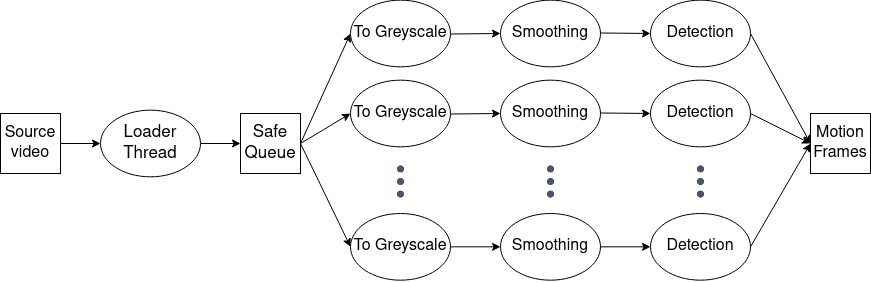
\includegraphics[width=0.85\textwidth]{img/par_code.png}
    \centering
    \caption{Scheme of the parallel implementation}
    \label{fig:par_code}
\end{figure}

In Figure \ref{fig:par_code}, we can see a scheme of the workflow of the standard C++ thread implementation.
All the computation is managed with \texttt{std::async}, using the \texttt{std::launch::async} policy to run the function on a new thread.

First of all, we have a \emph{Loader} thread, which reads each frame from the source video and stores them in a queue. This thread, in addition to the reference to the source video, receives a reference to the shared queue, which is initialized with a proper size, in order to not saturate the memory and hence getting killed by the system. The queue size is computed taking into consideration the size in bytes of the backgroud image and the memory available on the machine. Further details about the SafeQueue implementation are in section \ref{sec:safequeue}.

Then, we have a Farm made by \emph{nw} threads, in which each worker gets a frame from the shared queue and process it; each thread performs the work sequentially, using the methods defined in the sequential implementation.\\
Each thread creates two \texttt{cv::Mat} objects, a \texttt{grey\_frame} and a \texttt{smoothed\_frame}; both are defined having the same number of rows and columns as the original frame, but with a single channel.
The \texttt{grey\_frame} is needed to store the result of the \texttt{to\_greyscale()} operation, which cannot be performed \emph{in-place} because the original frame is defined to have three channels for the \emph{RGB} values.\\
Instead, for the \texttt{smoothing()} operation, we use the additional \texttt{smoothed\_frame} object to avoid the problems that arise from the \emph{in-place} application of a stencil pattern. Plus, we pay particular attention to the computation at the borders of the matrix, which can be problematic and can lead to errors; for this reason, we always check that the position we want to access is between 0 and the number of rows/columns of the frame.

At the end, when a worker executes the \texttt{motion\_detection()} method and if it returns \texttt{true}, it increases the value of a shared variable \texttt{motion\_frames}, which is defined as an \texttt{atomic<int>} to avoid problems concerning the concurrency on the write operation.

Finally, the code returns the number of frames with motion, the completion time expressed in microseconds and an average of the latency of the process, expressed in microseconds and computed as the ratio between the completion time and the number of frames processed.

\subsubsection{SafeQueue} \label{sec:safequeue}
SafeQueue is a class that defines a queue designed to be shared among threads, hiding the synchronization mechanism.\\
The constructor takes in input only the maximum size of the queue. Then, the two main methods are \texttt{push()} and \texttt{pop()}: the \texttt{push()} method takes in input an item, waits on a condition variable if the queue is full, inserts the item in the queue and notifies it to the other threads; the \texttt{pop()} method waits if the queue is empty, as long as the computation is not finished, then removes an item from the queue and returns it. These two operations are performed after acquiring a lock, to be sure to have only one thread modifying the queue at a time.

\subsection{FastFlow Implementation}
The FastFlow implementation is conceptually similar to the one provided with standard C++ threads. It exploits the \texttt{ff\_Farm} high-level pattern offered by the library; a simple representation of the architecture can be seen in Figure \ref{fig:ff_code}.

\begin{figure}[h]
    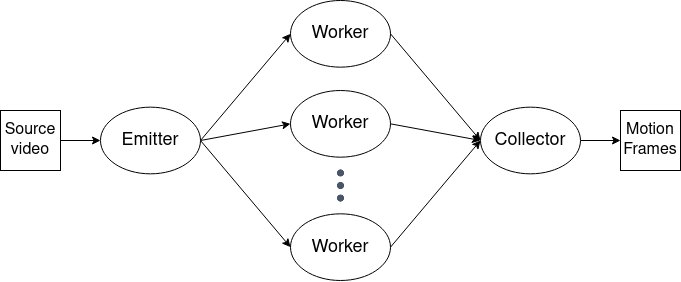
\includegraphics[width=0.85\textwidth]{img/ff_code.png}
    \centering
    \caption{Scheme of the FastFlow implementation}
    \label{fig:ff_code}
\end{figure}

Here we have an \emph{Emitter} node that loads the frames from the source video, stores each of them in a \texttt{cv::Mat*} and sends them through the method \texttt{ff\_send\_out()}. Using this function, the library pushes the loaded frames in the shared queues, so that the following workers can read them from there. When there are no more frames to read, the emitter returns the special value \texttt{EOS}, telling to the successive states that the computation has to be finished.

Then, there is a Farm of \emph{nw} threads, each one performing the work sequentially, in the same way as the standard thread implementation. Also in this case, the threads use two auxiliary \texttt{cv::Mat} objects, and they exploits the function defined in the sequential implementation.
Each thread return a \texttt{boolean} flag, indicating whether the current frame has motion or not.

This flag is passed to the \emph{Collector} node, which increases the value of the integer variable \texttt{motion\_frames}. In the end, the collector returns the special value \texttt{GO\_ON}, meaning that the node is ready to receive the next input.

Also this implementation returns the number of frames with motion, together with the completion time and the latency, expressed in microseconds.